% !TeX program = xelatex
\documentclass[11pt,a4paper]{article}
\usepackage{fontspec,polyglossia}
\setdefaultlanguage{russian}
\setotherlanguage{english}
\setmainfont[Path=fonts/,UprightFont=cmunrm.otf,BoldFont=cmunbx.otf,ItalicFont=cmunti.otf,BoldItalicFont=cmunbi.otf]{CMU Serif}
\newfontfamily\cyrillicfonttt[Path=fonts/]{cmuntt.otf}
\usepackage[a4paper,left=2cm,right=2cm,top=2cm,bottom=3cm]{geometry}
\usepackage{graphicx,longtable,booktabs,array,float,setspace,xurl,hyperref,pdflscape}
\hypersetup{unicode=true,colorlinks=true,linkcolor=black,urlcolor=blue,pdftitle={Лабораторная работа № 2. Импорт и транзакции},pdfauthor={Чэнь Хаолинь}}
\setlength{\parindent}{0cm}
\setlength{\parskip}{0.2\baselineskip}
\setlength{\emergencystretch}{3em}
\renewcommand{\arraystretch}{1.15}
\newcolumntype{L}[1]{>{\raggedright\arraybackslash}p{#1}}
\begin{document}
\hypersetup{pageanchor=false}
% !TeX encoding = UTF-8
\begin{titlepage}
\centering
Федеральное государственное автономное \\
образовательное учреждение высшего образования \\
\textbf{«Национальный исследовательский университет ИТМО»} \\
\vfill
Информационные системы\\
\vspace{0.5\baselineskip}
\textbf{Лабораторная работа № 2} \\
\vspace{0.5\baselineskip}
Импорт объектов и изоляция транзакций\\
Вариант 4101\\
\vfill
\begin{flushright}
Выполнил:\\
Чэнь Хаолинь P3316\\
Преподаватель:\\
Коновалов Арсений Антонович\\
\end{flushright}
\vspace{4\baselineskip}
\centering
г. Санкт-Петербург, 2026
\end{titlepage}

\hypersetup{pageanchor=true}
\tableofcontents\clearpage
\section{Задание}
Доработать ИС из ЛР1 следующим образом:


1. Добавить в систему возможность массового добавления объектов при помощи импорта файла. Формат для импорта необходимо согласовать с преподавателем. Импортируемый файл должен загружаться на сервер через интерфейс разработанного веб-приложения.


- При реализации логики импорта объектов необходимо реализовать транзакцию таким образом, чтобы в случае возникновения ошибки при импорте не был создан ни один объект.


- При импорте должна быть реализована проверка пользовательского ввода в соответствии с ограничениями предметной области из ЛР1.


- При наличии вложенных объектов в основном объекте из ЛР1 необходимо задавать значения полей вложенных объектов в той же записи, что и основной объект.


2. Необходимо добавить в систему интерфейс для отображения истории импорта (обычный пользователь видит только операции импорта, запущенные им, администратор — все операции).


- В истории должны отображаться ID операции, статус её завершения, пользователь, который её запустил, число добавленных объектов в операции (только для успешно завершённых).


3. Согласовать с преподавателем и добавить в модель из первой лабораторной новые ограничения уникальности, проверяемые на программном уровне (эти новые ограничения должны быть реализованы в рамках бизнес-логики приложения и не должны быть отображены/реализованы в БД).


4. Реализовать сценарий с использованием Apache JMeter, имитирующий одновременную работу нескольких пользователей с ИС, и проверить корректность изоляции транзакций, используемых в ЛР. По итогам исследования поведения системы при её одновременном использовании несколькими пользователями изменить уровень изоляции транзакций там, где это требуется. Обосновать изменения.


- Реализованный сценарий должен покрывать создание, редактирование, удаление и импорт объектов.


- Реализованный сценарий должен проверять корректность поведения системы при попытке нескольких пользователей обновить и/или удалить один и тот же объект (например, двух администраторов).


- Реализованный сценарий должен проверять корректность соблюдения системой ограничений уникальности предметной области при одновременной попытке нескольких пользователей создать объект с одним и тем же уникальным значением.


\subsection{Требования к отчёту}
\begin{enumerate}\setlength{\itemsep}{0pt}
\item Текст задания.
\item UML-диаграммы классов и пакетов разработанного приложения.
\item Исходный код системы или ссылка на репозиторий с исходным кодом.
\item Выводы по работе.
\end{enumerate}

\subsection{Вопросы к защите}
\begin{enumerate}\setlength{\itemsep}{0pt}
\item Понятие бизнес-логики в программных системах. Уровень бизнес-логики в многоуровневой архитектуре программных систем.
\item Jakarta Enterprise Beans (EJB). Виды бинов и их назначение.
\item EJB Session beans. Жизненный цикл.
\item Понятие транзакции. Транзакции в БД. ACID.
\item Виды конфликтов при многопользовательской работе с данными. Уровни изоляции транзакций.
\item Особенности реализации транзакций на уровне бизнес-логики, отличия от транзакций на уровне БД.
\item Java Transaction API. Основные принципы и программные интерфейсы.
\item Реализация управления транзакциями в Jakarta EE. Декларативное и программное управление транзакциями.
\item Реализация управления транзакциями в Spring. Декларативное и программное управление транзакциями в Spring. Аннотация \texttt{@Transactional}.
\end{enumerate}

\subsection{Принятые решения}
С преподавателем согласованы формат JSON и уникальность сочетания названия фильма и режиссёра, реализуемая только в бизнес-логике приложения. Система развивает приложение первой лабораторной работы и сохраняет операции CRUD и специальные операции.
\section{Реализация}
\subsection{Архитектура и модель данных}
Приложение использует Jakarta EE 10: CDI управляет компонентами бизнес-логики, Jakarta REST обслуживает API, Jakarta Persistence и EclipseLink работают с PostgreSQL. Пользовательский интерфейс реализован средствами HTML, CSS и JavaScript. Транзакции имеют тип \texttt{RESOURCE\_LOCAL}; их границы заданы программно через \texttt{EntityTransaction}. Аннотация \texttt{@Transactional} в данной реализации не используется.

К существующим сущностям добавлены \texttt{ImportOperation}, состояния \texttt{RUNNING}, \texttt{SUCCESS}, \texttt{FAILED} и роли \texttt{USER}, \texttt{ADMIN}. История связана с учётной записью по идентификатору. В API возвращается безопасное представление: идентификатор операции, пользователь, статус, число добавленных фильмов только при успехе, время, имя файла и краткая причина ошибки. Пароли, соли и хеши в него не входят.

Миграция \path{003_lab2_roles_imports.sql} сохраняет существующие строки и назначает прежним пользователям роль USER. Повторное выполнение безопасно. Регистрация всегда создаёт обычного пользователя; роль администратора назначается серверным скриптом по точному имени уже зарегистрированной учётной записи.

\subsection{Формат импорта и проверка данных}
Файл передаётся на сервер как \path{multipart/form-data}, поле \texttt{file}, тип содержимого \path{application/json}. Браузер отправляет исходный объект File без преобразования JSON в JavaScript Number. Сохраняются Session Cookie и защита CSRF. Приняты ограничения 5 MiB и 1000 фильмов; пустой массив запрещён.

Верхний объект содержит целочисленный \texttt{formatVersion=1} и массив \texttt{movies}. Coordinates, Person и Location задаются вложенными объектами той же записи. Парсер проверяет UTF-8, допускает начальный BOM, отклоняет неизвестные и повторные свойства, автоматически формируемые поля, неверные типы, дробные значения целых полей, переполнение и неконечные числа. Long разбирается точно из целого JSON или десятичной строки; значение 9007199254740993 не проходит через Double. После разбора выполняется та же Bean Validation, что и при CRUD.

Для каждой записи создаются новые координаты. Человек определяется по уникальному \texttt{passportID}. Если человек уже существует, все его переданные поля должны совпадать; Location сравнивается по значениям, ZonedDateTime --- с учётом часового пояса, числа --- после преобразования в соответствующий Java-тип. Несовпадение вызывает \texttt{PERSON\_DATA\_CONFLICT}; импорт никогда не редактирует существующего человека неявно.

\subsection{Новая уникальность}
Бизнес-ключ имеет два независимых компонента: точное сохранённое название и \texttt{Person.id} режиссёра либо null. Регистр, пробелы и Unicode не нормализуются. Одноимённые люди с разными идентификаторами являются разными режиссёрами. Два фильма с одинаковым названием и отсутствующим режиссёром считаются дубликатами. Изменение имени или паспорта человека не меняет его идентификатор.

\texttt{MovieUniquenessValidator} используется обычным созданием, частичным обновлением и импортом. Обновление сначала объединяет входные поля с существующей сущностью и исключает собственный ID из поиска. Сравнение названия через Java String.equals обеспечивает точную семантику. Для нового сочетания в PostgreSQL отсутствуют UNIQUE, уникальные индексы и триггеры; прежние ограничения паспорта и имени пользователя сохранены.

\subsection{Транзакции и обработка отказов}
После проверки аутентификации, CSRF, наличия, размера и типа файла короткая транзакция T1 сохраняет RUNNING. Затем сервер разбирает файл. Транзакция T2 сначала блокирует строку \texttt{AppState(id=1)} через \texttt{PESSIMISTIC\_WRITE}; все окончательные чтения, проверки версий и уникальности выполняются после получения этой блокировки. Все вложенные объекты и фильмы сохраняются в T2. SUCCESS и фактическое число фильмов фиксируются в той же транзакции; revision увеличивается один раз.

При ошибке T2 полностью откатывается. Независимая транзакция T3 сохраняет FAILED с пустым addedCount; история не исчезает вместе с объектами. Исторические транзакции не изменяют revision. Flush не является commit. Это существенно при IDENTITY: фактические INSERT могут выполняться до конца обработки файла, но остаются частью одной транзакции.

При неопределённом исходе commit новая связь с БД сначала проверяет историю. Уже подтверждённый SUCCESS не заменяется на FAILED. При недоступности проверки операция остаётся RUNNING; клиент получает идентификатор и указание проверить историю, без автоматической повторной загрузки. После остановки прежнего единственного экземпляра скрипт запуска проверяет процесс, получает блокировку AppState и восстанавливает оставшиеся RUNNING. Этот порядок предназначен для одного экземпляра приложения.

SQLSTATE 55P03, 57014 и известные временные ошибки отделены от бизнес-конфликтов; неожиданный сбой не выдаётся за допустимый 409. Для явно отменённых транзакций SERIALIZABLE предусмотрено не более трёх повторов с новым EntityManager. Пользовательские ошибки и конфликты версий не повторяются.

\subsection{Веб-интерфейс}
Добавлены страницы импорта и истории. Во время отправки повторный щелчок отключён; результат показывает ID операции, число фильмов либо код, номер записи и путь поля. История имеет собственный опрос, поэтому неуспешный импорт виден без изменения revision. Обычный пользователь видит свои операции, администратор --- все; проверка принадлежности выполняется сервером и для списка, и для отдельной записи.

По требованию пользователя итоговый интерфейс полностью русскоязычный; переключатель языка и номер варианта в верхней части страницы удалены. Механизм синхронизации первой работы сохранён: открытая форма оставляет пользовательский ввод и первоначальную версию, а сервер отклоняет устаревшее сохранение.

\section{UML-диаграммы}
Диаграммы отражают окончательные сущности и компоненты приложения. Редактируемые исходники Graphviz DOT, изображения SVG/PNG/PDF и контрольные суммы Java-файлов находятся в каталоге \path{report/Lab2/uml/}.

\begin{figure}[H]\centering
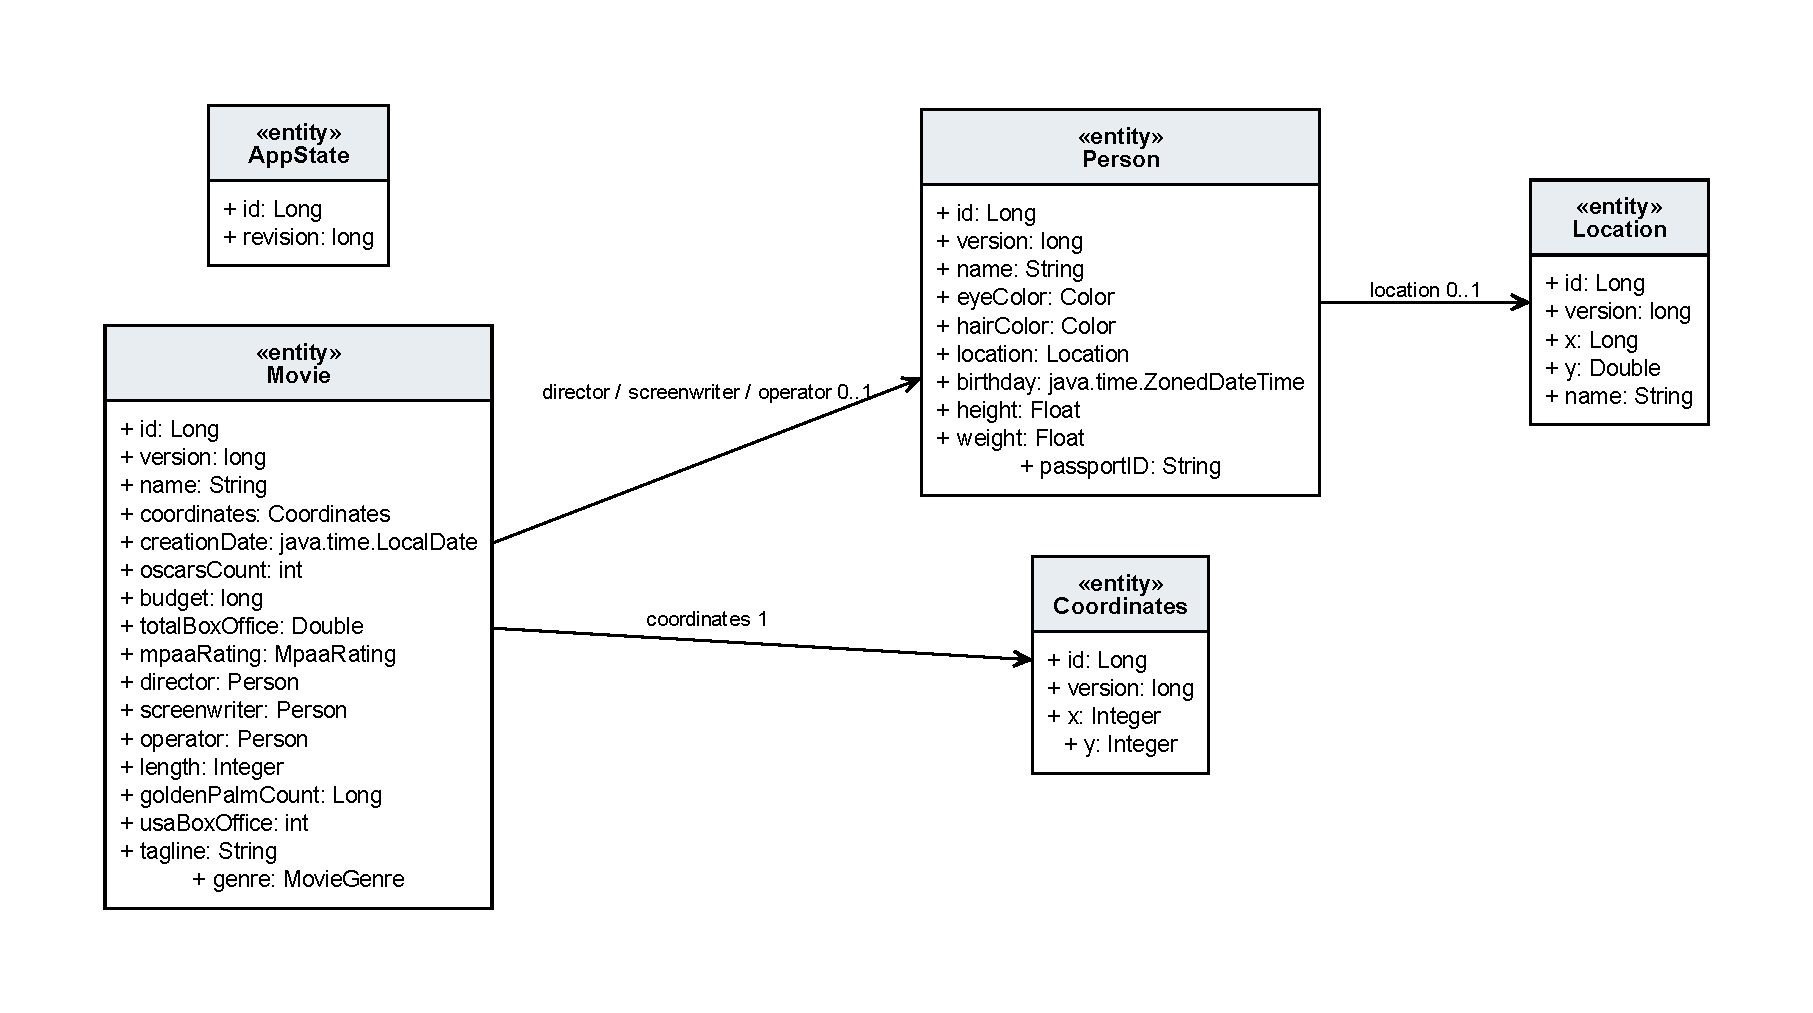
\includegraphics[width=\textwidth,height=0.72\textheight,keepaspectratio]{uml/classes-domain.pdf}
\caption{Классы предметной области и связи с вложенными объектами}
\end{figure}
\begin{figure}[H]\centering
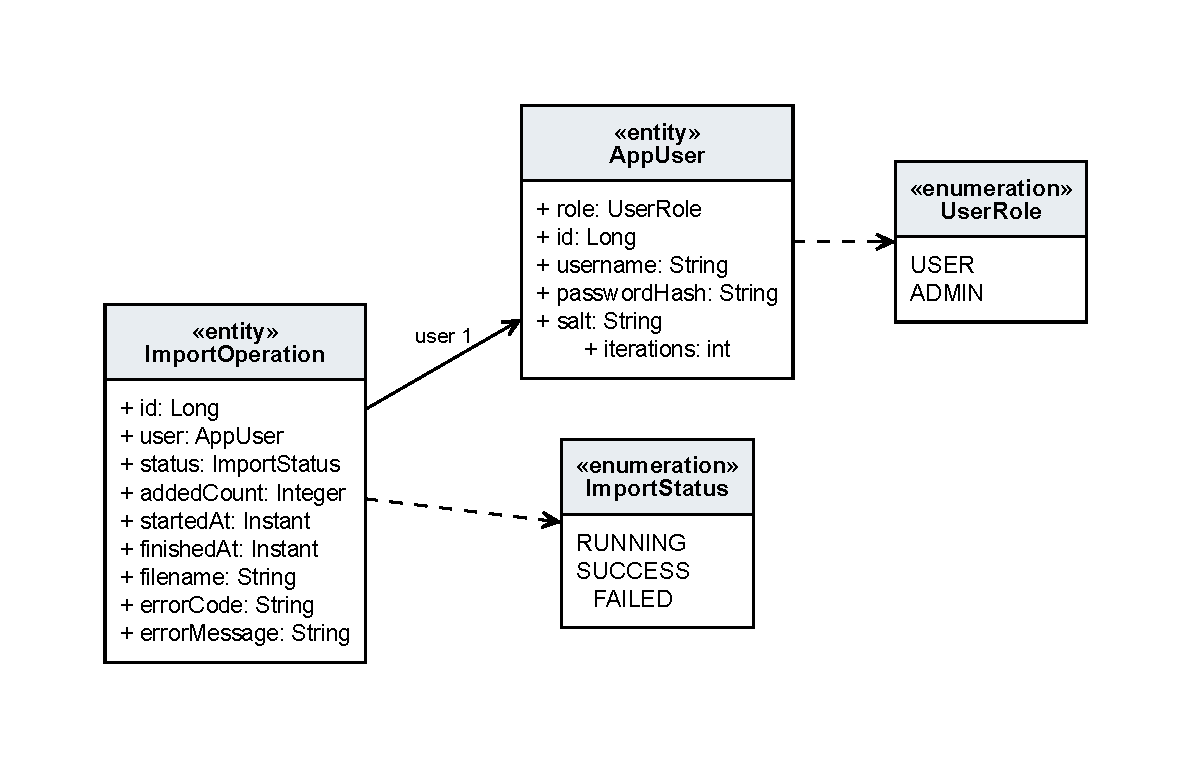
\includegraphics[width=\textwidth,height=0.65\textheight,keepaspectratio]{uml/classes-history.pdf}
\caption{Учётные записи, роли и устойчивое состояние импорта}
\end{figure}
\begin{landscape}
\begin{figure}[p]\centering
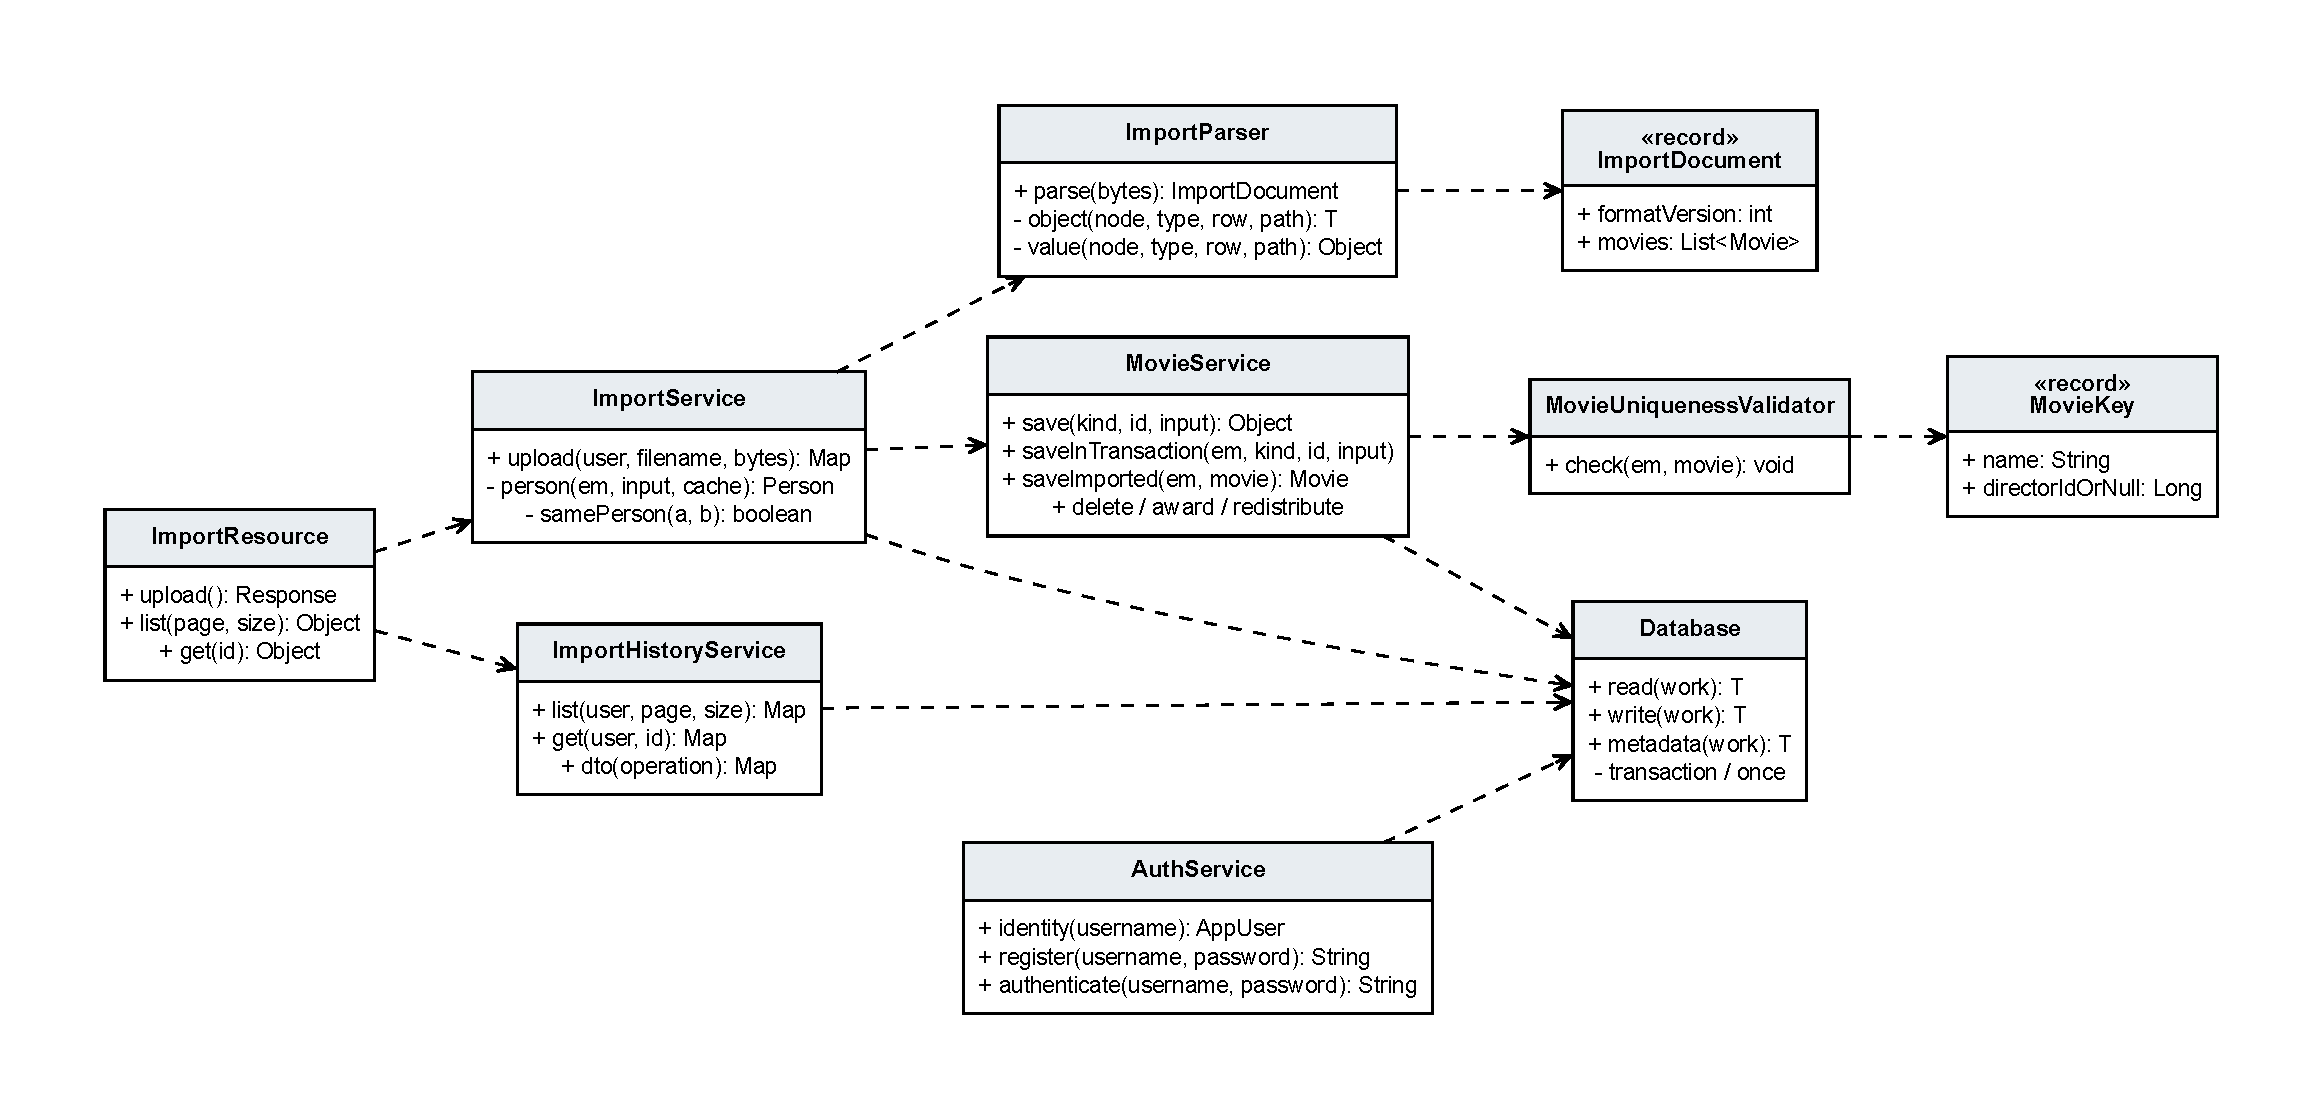
\includegraphics[width=\linewidth,height=0.85\textheight,keepaspectratio]{uml/classes-services.pdf}
\caption{Компоненты импорта, DTO и транзакционная граница}
\end{figure}
\end{landscape}
\begin{figure}[H]\centering
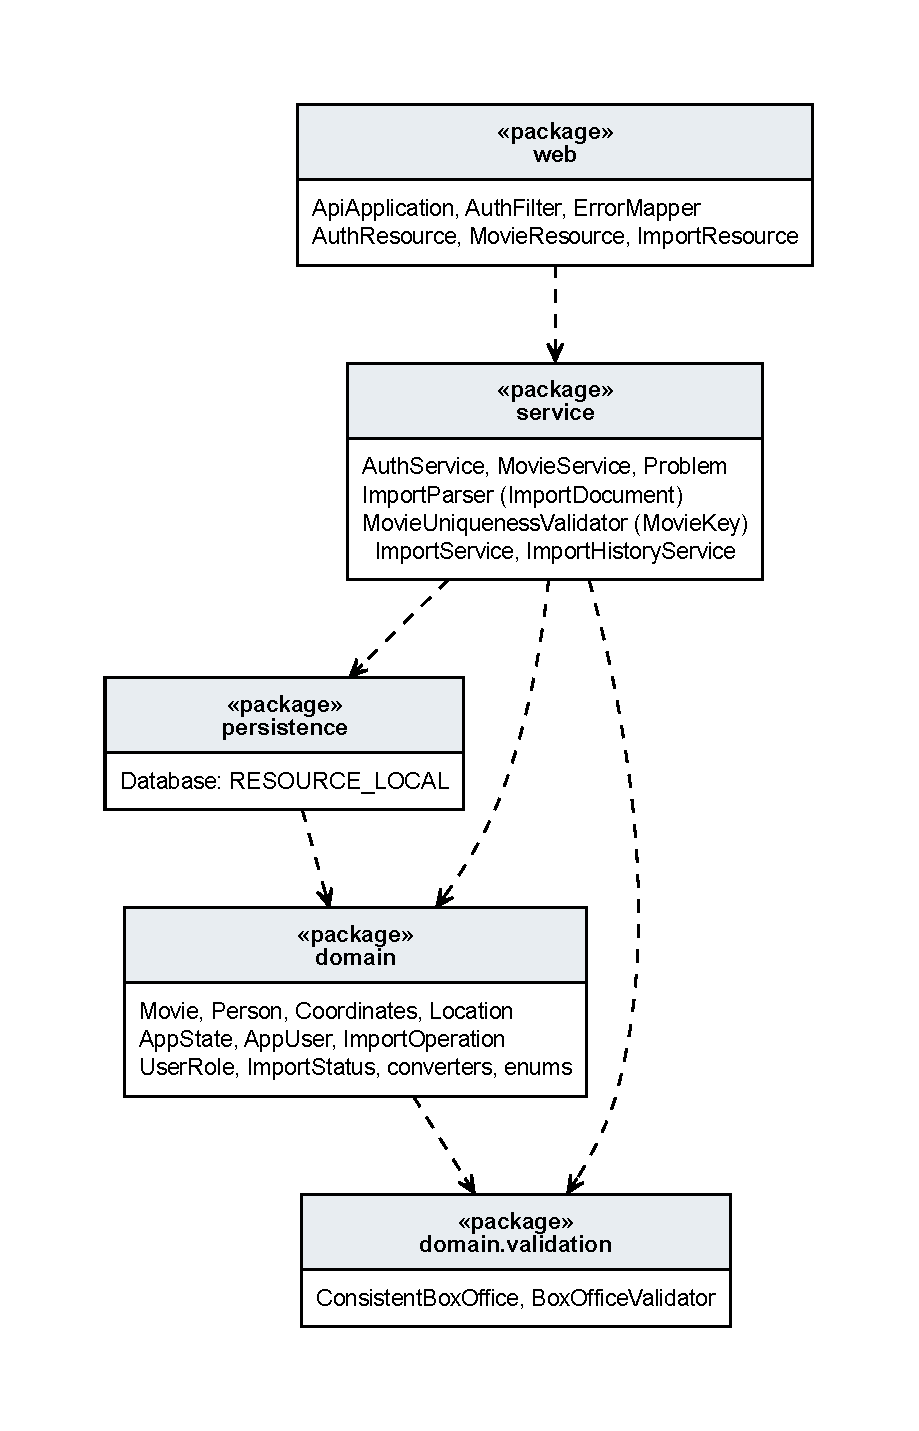
\includegraphics[width=\textwidth,height=0.65\textheight,keepaspectratio]{uml/packages.pdf}
\caption{Пакеты приложения и зависимости}
\end{figure}

\section{Проверка на Helios}
Среда: FreeBSD 14.5-STABLE, OpenJDK 21.0.4, Maven 3.8.4, PostgreSQL 18.3, Payara Micro 6.2025.1 и Apache JMeter 5.6.3. JUnit использует EclipseLink 4.0.5; в развёрнутом Payara фактически загружен контейнерный EclipseLink 4.0.1.payara-p3, что подтверждено журналом реальной транзакции. Серверные команды выполняются в \path{/home/studs/s407960/is-lab2-4101}. Экспериментальные таблицы имеют префикс \texttt{lab2\_4101\_test\_}; исходные таблицы первой работы не изменялись.

Первоначальная серверная проверка выявила отсутствующую persistence unit \texttt{movies-helios-test}. После добавления изолированных отображений сервер выполнил Maven clean verify: 140 тестов, 0 ошибок, 0 неуспешных, 0 пропущенных. Отдельные проверки воспроизводят исключение после реального insert/flush и ошибку отложенного ограничения при commit; в обоих случаях все четыре типа предметных объектов откатываются, а FAILED сохраняется.

Миграция дважды применена к независимой копии 32 фильмов и 3 учётных записей первой работы. Числа строк и хеши их содержимого совпали до и после; все существующие учётные записи получили роль USER. Семнадцать проверок HTTP подтвердили multipart, размеры, тип содержимого, CSRF, запрет самоназначения ADMIN и разграничение истории.

\subsection{Сценарии JMeter}
\begin{longtable}{lrrrrr}
\toprule Сценарий & Потоки & Раунды & Запросы & Commit & 409/404\\\midrule
C01 & 2 & 20 & 40 & 20 & 20\\
C02 & 2 & 20 & 40 & 20 & 20\\
C02D & 2 & 20 & 40 & 20 & 20\\
C03 & 10 & 20 & 200 & 20 & 180\\
C04 & 10 & 20 & 200 & 20 & 180\\
C05 & 10 & 20 & 200 & 200 & 0\\
C06 & 2 & 20 & 40 & 20 & 20\\
C07 & 10 & 20 & 200 & 20 & 180\\
C08 & 2 & 20 & 40 & 20 & 20\\
C09 & 2 & 20 & 40 & 20 & 20\\
C10 & 10 & 20 & 200 & 180 & 20\\
C11 & 10 & 20 & 200 & 20 & 0\\
C12 & 10 & 20 & 200 & 200 & 0\\
\bottomrule\end{longtable}
Все 13 вариантов (включая C02D) выполнили по 20 раундов. Всего 1640 целевых запросов: 780 зафиксированных изменений, 680 ожидаемых бизнес-конфликтов и 180 чтений. Неожиданных отказов, дубликатов ключа, остатков неуспешного импорта и ошибок JTL не обнаружено. Проверялись конечные значения и версии, все четыре типа предметных объектов, статусы и счётчики истории. C11 дополнен детерминированным серверным JUnit с паузой после flush.

\subsection{Исследование изоляции}
\begin{longtable}{L{7cm}rr}

\toprule Показатель & READ COMMITTED & SERIALIZABLE\\\midrule

Целевые запросы, фактически & 1640 & 1070\\

Зафиксированные изменения & 780 & 225\\

Ожидаемые конфликты & 680 & 661\\

Неожиданные отказы & 0 & 4\\

Повторы сериализации & 0 & 517\\

Дубликаты / остатки импорта & 0 / 0 & 0 / 0\\

\bottomrule\end{longtable}

Обе группы использовали один WAR и один восстановленный снимок тестовых таблиц, одинаковый AppState lock, число потоков и предел трёх повторов 40001. При SERIALIZABLE сценарии C05, C10 и C12 остановлены после первого раунда из-за исчерпания повторов и ответа 503; оставшиеся 19 раундов не выполнены и не засчитаны. Отсутствие дубликатов при этом не означает успешность сценария.

Окончательно сохранён READ COMMITTED, заданный явно в бизнес-транзакциях. Глобальная строка-блокировка сериализует окончательные проверки и запись, а ожидаемая версия защищает старую пользовательскую форму. Повышение изоляции при том же глобальном lock не улучшило проверяемые инварианты, но вызвало дополнительные отказы. Короткие транзакции истории также используют READ COMMITTED и не изменяют revision.

Уровень прочитан через SHOW transaction\_isolation в настоящем соединении Database.write и в отдельной транзакции metadata. Ограничение ожидания 200 ms реально дало 55P03 через 217 ms; стандартный Web-порог 10000 ms дал 503 примерно через 10,038 s. Шум общей машины и ранняя остановка не позволяют сравнивать агрегированные времена как строгий benchmark.

Не выполнялась инъекция сетевого разрыва точно в момент ответа commit и нагрузка импортом максимальных 1000 строк. Проверка восстановления RUNNING использует явно созданную изолированную запись и реальный перезапуск единственного процесса; многопроцессное восстановление не заявляется.

\subsection{Проверка в браузере}
Браузер обращается через SSH-туннель \texttt{127.0.0.1:18083} к серверному \texttt{127.0.0.1:40797}. Успешная загрузка выполнена выбором настоящего JSON-файла; повторная загрузка отклонена. Два независимых Cookie-контекста подтвердили видимость истории по ролям и конфликт старой формы после изменения в другой сессии. Ниже приведены снимки первоначальной серверной проверки; последующая правка интерфейса описана отдельно.
\begin{figure}[H]\centering
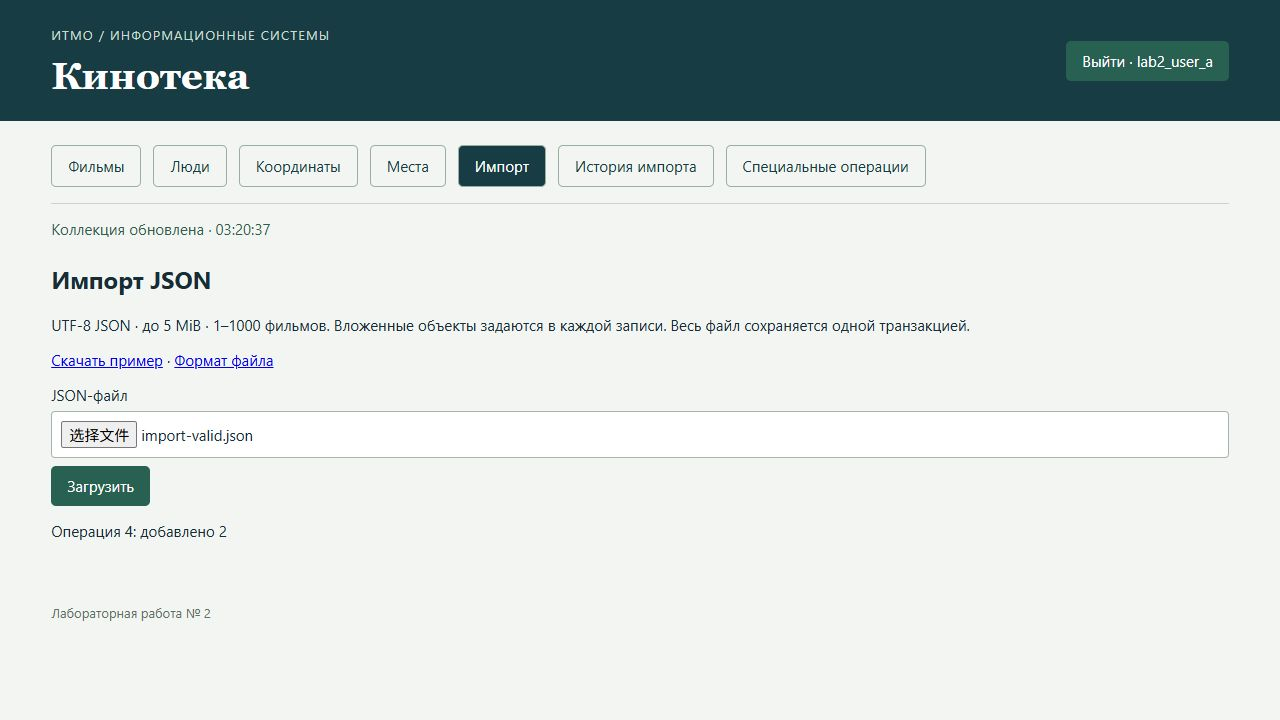
\includegraphics[width=\textwidth]{images/final-import-success.png}
\caption{Загрузка настоящего JSON-файла: два фильма сохранены в формальной установке на Helios}
\end{figure}
\begin{figure}[H]\centering
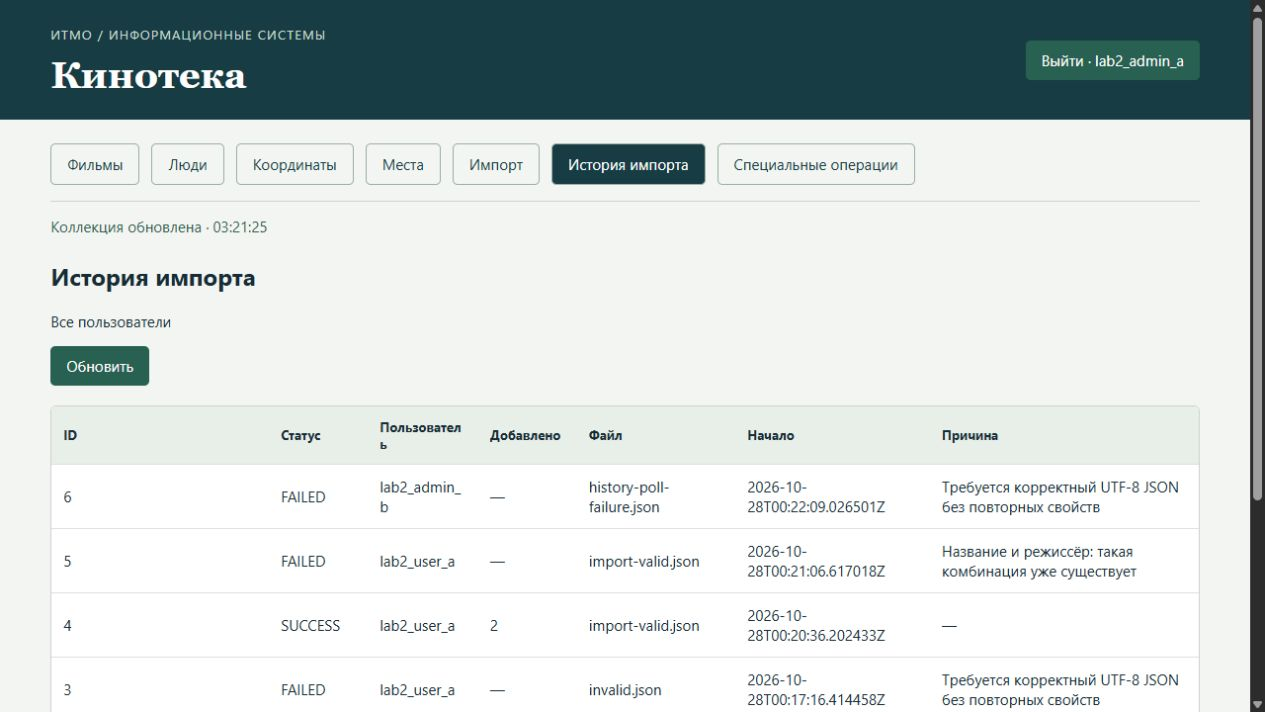
\includegraphics[width=\textwidth]{images/final-history-admin.png}
\caption{Администратор видит операции разных пользователей; FAILED не показывает число объектов}
\end{figure}
\begin{figure}[H]\centering
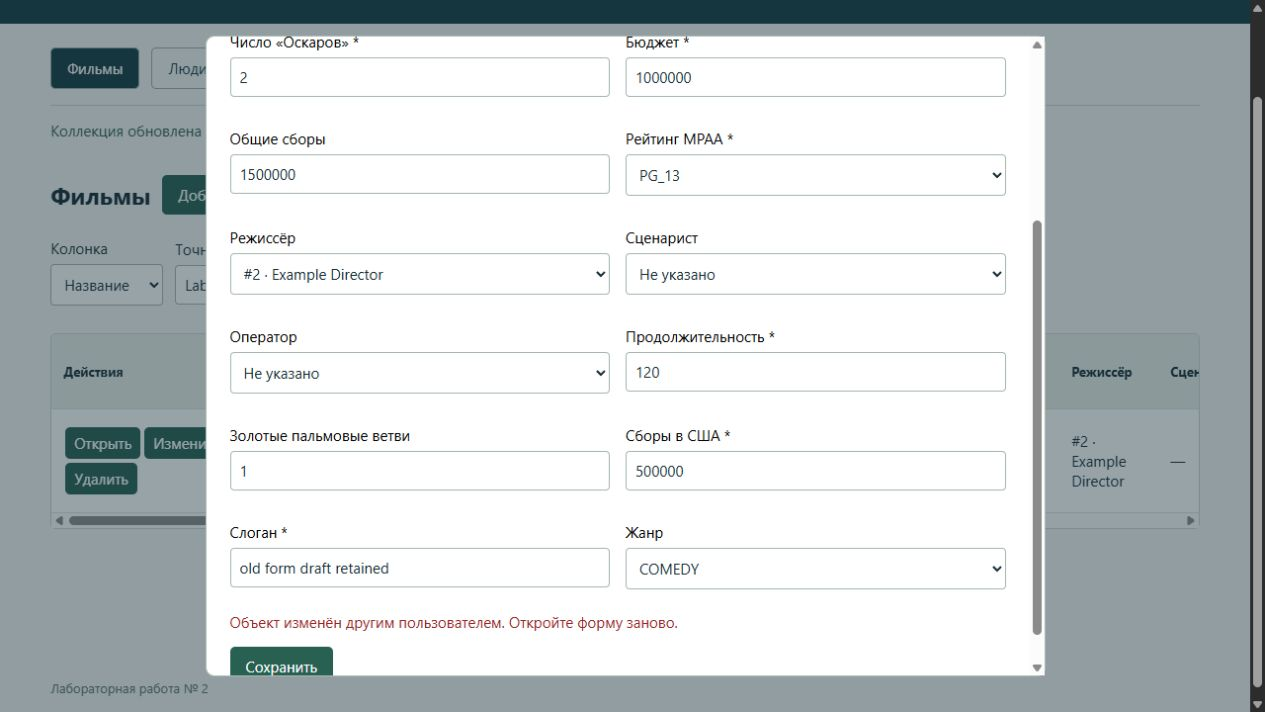
\includegraphics[width=\textwidth]{images/final-stale-edit-conflict.png}
\caption{Старая форма сохраняет черновик и получает конфликт версии вместо перезаписи чужого изменения}
\end{figure}


\subsection{Формальная установка и перезапуск}
Исходный проверенный WAR развёрнут с persistence unit \texttt{movies-helios} на продуктивных таблицах \texttt{lab2\_4101\_}; его SHA-256 совпадает с артефактом обоих окончательных прогонов JMeter. Семнадцать HTTP-проверок повторены на этих таблицах. Прямой снимок PostgreSQL совпадает с объектами API. Хеши исходных таблиц первой работы совпадают с исходным состоянием.

При настоящем перезапуске процесса сохранены четыре проверяемые учётные записи, их роли, фильмы и терминальные записи истории. Отдельная явно созданная SQL-запись RUNNING восстановлена в FAILED; это контрольная запись для проверки recovery, а не утверждение о реально произошедшем неопределённом commit. После обнаруженного выхода прежнего процесса в 05:00 сервис возобновлён тем же WAR; повторно проверены сохранность данных и статусов. Причина выхода из одного журнала приложения не установлена.

После замечаний к интерфейсу на Helios выполнен новый Maven package: изменены четыре веб-файла, остальные записи WAR побайтово совпадают. Выбор файла теперь имеет русские надписи; две подсказки и кнопка обновления удалены. Проверены реальная загрузка, автоматическое появление FAILED без изменения revision и пагинация. Полные JUnit/JMeter повторно не запускались. Доказательства: \path{verification/Lab2/ui-review/} и \path{verification/Lab2/browser/final-ui-checks.json}.

\section{Исходный код и воспроизведение}
Каталог \path{movie-lab/} содержит полный код, миграции, JSON-примеры и JMeter-сценарии. Вместе с отчётом поставляются \href{../../verification/Lab2/source-final.tar.gz}{архив исходников} и \href{../../movie-lab/source-manifest.json}{манифест SHA-256}. Команды воспроизведения приведены в \path{movie-lab/README.md} и \path{movie-lab/jmeter/README.md}, результаты и ограничения --- в \path{verification/Lab2/ACCEPTANCE.md}. JTL, HTML, сырые ответы и снимки БД сохранены для каждого прогона. Пароли, частные дампы и сессионные токены исключены.

\section{Заключение}
В приложении первой лабораторной работы реализованы атомарный JSON-импорт, сохранение истории с разграничением USER/ADMIN и программная уникальность сочетания точного названия и идентификатора режиссёра, включая null. Новая уникальность не перенесена в ограничения PostgreSQL. Транзакционные границы подтверждены реальным откатом после insert/flush и при отложенной ошибке commit.

На Helios успешно выполнены 140 серверных тестов и окончательный JMeter-прогон всех сценариев: 1640 целевых запросов без неожиданных отказов, дубликатов и остатков неуспешного импорта. Два браузерных сеанса через SSH-туннель подтвердили загрузку файла, синхронизацию, права истории и конфликт устаревшей формы. После правок интерфейса серверный код побайтово сохранён; исходные данные первой работы не изменены.

READ COMMITTED оставлен с явной настройкой, глобальным AppState lock и проверкой версий. При том же WAR и начальном снимке SERIALIZABLE дал 517 повторов и четыре неожиданных отказа, не улучшив проверяемые инварианты. Неисполненные после остановки раунды не засчитаны. Предельная нагрузка в 1000 записей и сетевой разрыв точно в момент commit не проверялись; восстановление рассчитано на один экземпляр. Эти ограничения отделены от фактически подтверждённых результатов.


\end{document}
